\subsection{A fictitious perfect cache}
In our first analysis we look at our four investigations from a first seen / last seen event perspective. We define a model where a fictitious perfect infinite cache is used. Every time a piece of data is first seen, its data size is added to the cache. Every time its last seen its removed out of the cache. ~\ref{fig:VirtCacheSize} on page ~\pageref{fig:VirtCacheSize} shows the probability density function of the required amount of RAM to implement such a perfect disk cache in.The X axis is the $\log{\Delta C}$ where $C$ is the size of the fictitious cache size at any point in time during an active OCFA run. When we look at ~\ref{fig:VirtCacheSize}, we see some quite different results depending on the investigation. While for example a fictitious cache size of $10^9$ (1 GB) would fit all active data for about 65\% of the time for investigation 1, the same amount would yield a fit for only one or two percent of the time in investigation 3. One main conclusion that we can draw from three out of four investigations is that most still active data could not possibly stay contained in any reasonable amount physical RAM memory that the OCFA machines might have had. In the following sub sections we discuss why this is the case.
\begin{figure}
\centering
\subfloat[case 1]{
  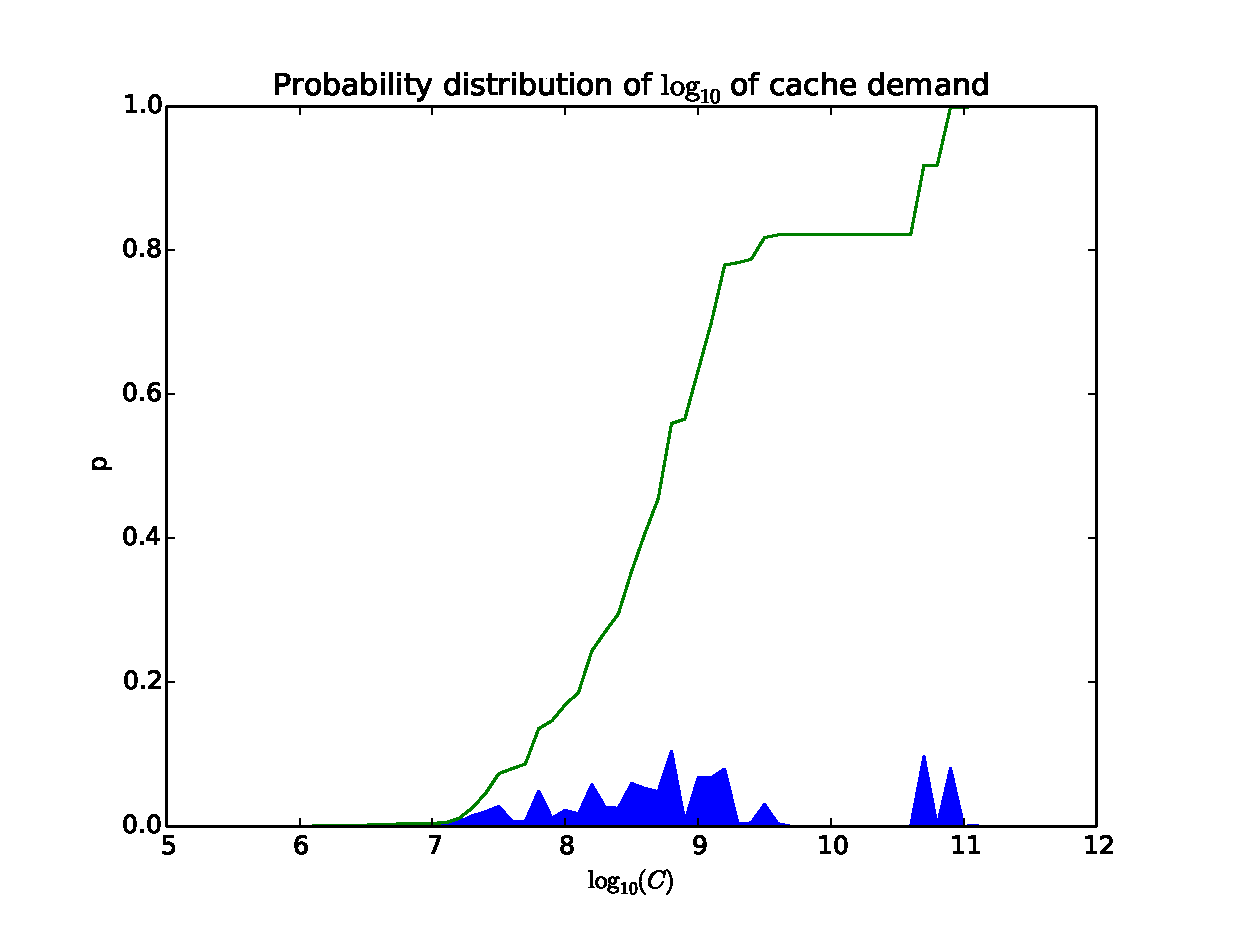
\includegraphics[width=70mm]{ocfa/step2/stripped1_virtcachesize.eps}
}
\subfloat[case 2]{
  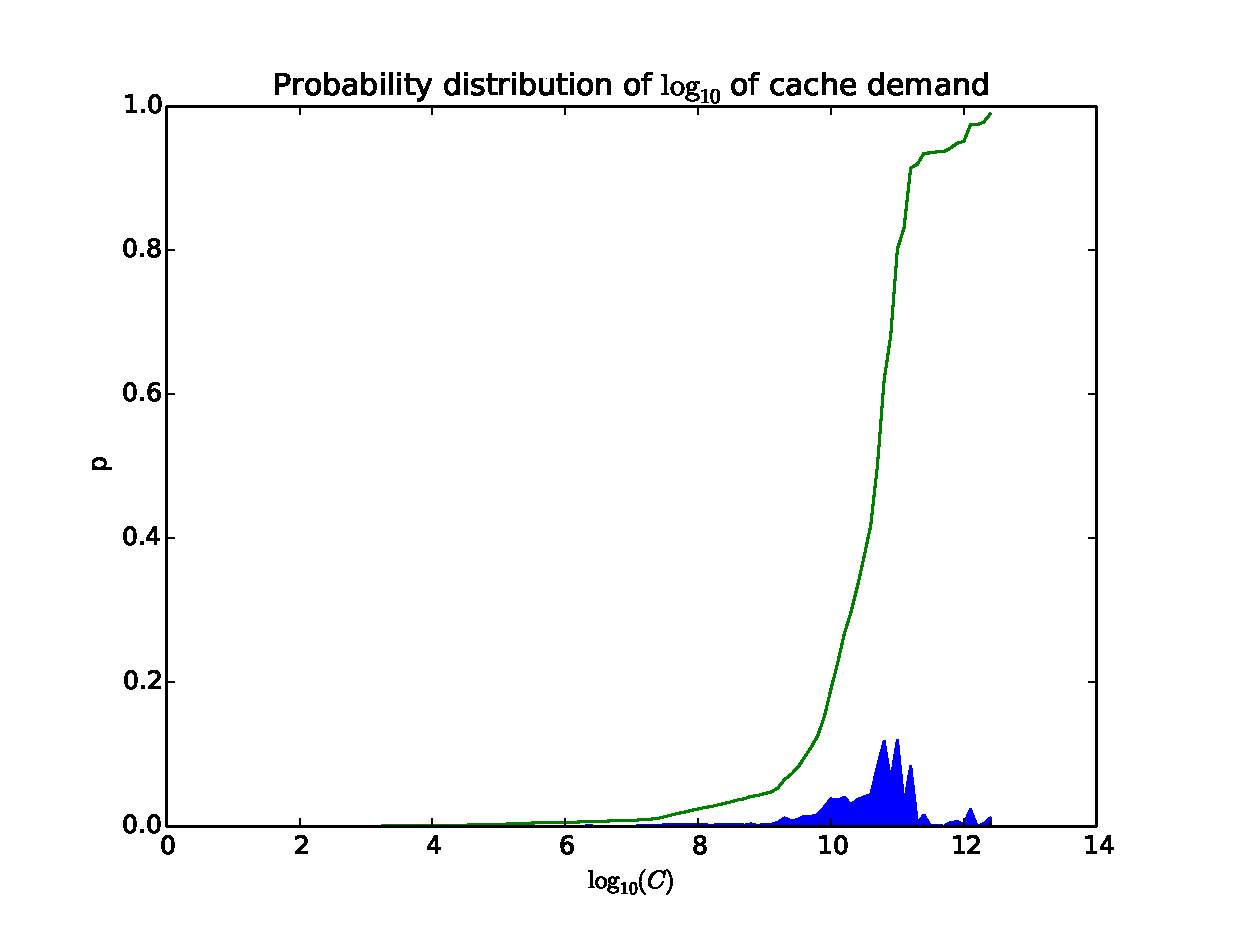
\includegraphics[width=70mm]{ocfa/step2/stripped2_virtcachesize.eps}
}
\hspace{0mm}
\subfloat[case 3]{
  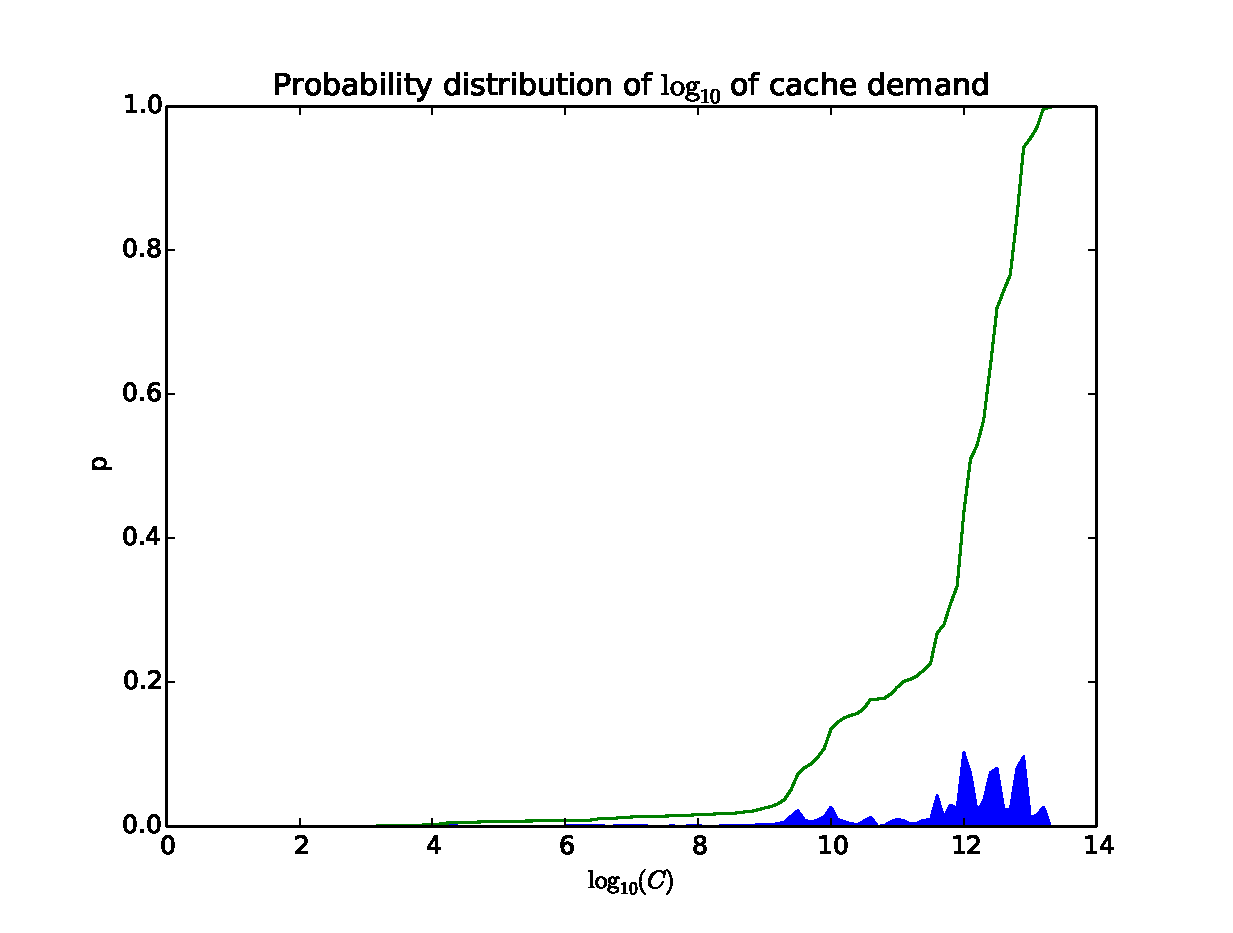
\includegraphics[width=70mm]{ocfa/step2/stripped3_virtcachesize.eps}
}
\subfloat[case 4]{
  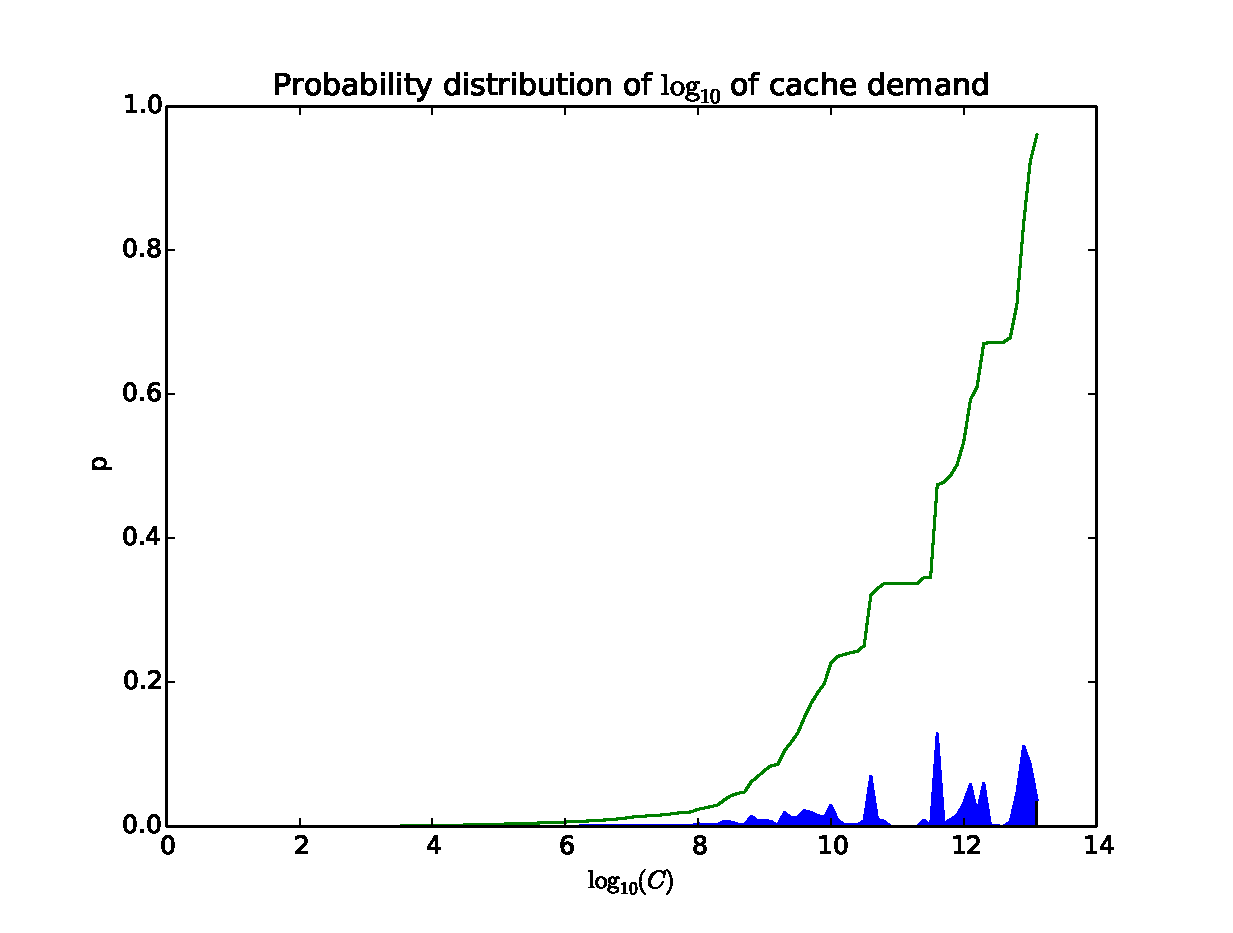
\includegraphics[width=70mm]{ocfa/step2/stripped4_virtcachesize.eps}
}
\caption{Virtual cache size probability density}
\label{fig:VirtCacheSize}
\end{figure}
